
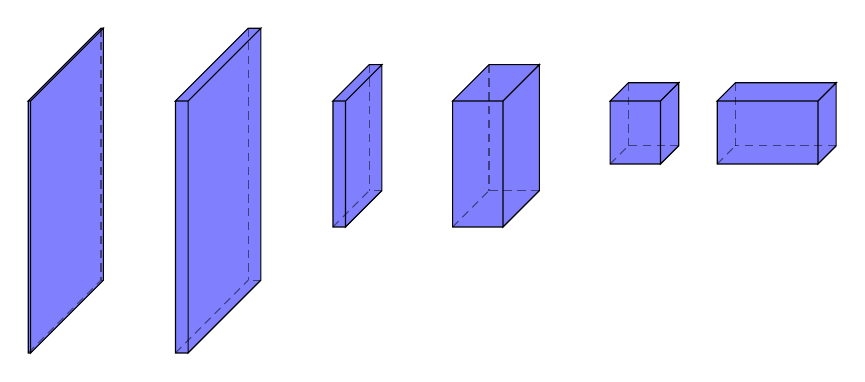
\begin{tikzpicture}[every edge quotes/.append style={auto, text=blue}]
\pgfmathsetmacro{\cubex}{0.03}
\pgfmathsetmacro{\cubey}{3.20}
\pgfmathsetmacro{\cubez}{2.40}
\draw [draw=black, every edge/.append style={draw=black, densely dashed, opacity=.5}, fill=blue!50]
(0,0,0) coordinate (o) -- ++(-\cubex,0, 0) coordinate (a) -- ++(0,-\cubey,0) coordinate (b) edge coordinate [pos=1] (g) ++(0,0,-\cubez)  -- ++(\cubex,0,0) coordinate (c) -- cycle
(o) -- ++(0,0,-\cubez) coordinate (d) -- ++(0,-\cubey,0) coordinate (e) edge (g) -- (c) -- cycle
(o) -- (a) -- ++(0,0,-\cubez) coordinate (f) edge (g) -- (d) -- cycle;

\pgfmathsetmacro{\cubex}{0.16}
\pgfmathsetmacro{\cubey}{3.20}
\pgfmathsetmacro{\cubez}{2.40}
\draw [draw=black, every edge/.append style={draw=black, densely dashed, opacity=.5}, fill=blue!50]
(2,0,0) coordinate (o) -- ++(-\cubex,0, 0) coordinate (a) -- ++(0,-\cubey,0) coordinate (b) edge coordinate [pos=1] (g) ++(0,0,-\cubez)  -- ++(\cubex,0,0) coordinate (c) -- cycle
(o) -- ++(0,0,-\cubez) coordinate (d) -- ++(0,-\cubey,0) coordinate (e) edge (g) -- (c) -- cycle
(o) -- (a) -- ++(0,0,-\cubez) coordinate (f) edge (g) -- (d) -- cycle;

\pgfmathsetmacro{\cubex}{0.16}
\pgfmathsetmacro{\cubey}{1.60}
\pgfmathsetmacro{\cubez}{1.20}
\draw [draw=black, every edge/.append style={draw=black, densely dashed, opacity=.5}, fill=blue!50]
(4,0,0) coordinate (o) -- ++(-\cubex,0, 0) coordinate (a) -- ++(0,-\cubey,0) coordinate (b) edge coordinate [pos=1] (g) ++(0,0,-\cubez)  -- ++(\cubex,0,0) coordinate (c) -- cycle
(o) -- ++(0,0,-\cubez) coordinate (d) -- ++(0,-\cubey,0) coordinate (e) edge (g) -- (c) -- cycle
(o) -- (a) -- ++(0,0,-\cubez) coordinate (f) edge (g) -- (d) -- cycle;

\pgfmathsetmacro{\cubex}{0.64}
\pgfmathsetmacro{\cubey}{1.60}
\pgfmathsetmacro{\cubez}{1.20}
\draw [draw=black, every edge/.append style={draw=black, densely dashed, opacity=.5}, fill=blue!50]
(6,0,0) coordinate (o) -- ++(-\cubex,0, 0) coordinate (a) -- ++(0,-\cubey,0) coordinate (b) edge coordinate [pos=1] (g) ++(0,0,-\cubez)  -- ++(\cubex,0,0) coordinate (c) -- cycle
(o) -- ++(0,0,-\cubez) coordinate (d) -- ++(0,-\cubey,0) coordinate (e) edge (g) -- (c) -- cycle
(o) -- (a) -- ++(0,0,-\cubez) coordinate (f) edge (g) -- (d) -- cycle;

\pgfmathsetmacro{\cubex}{0.64}
\pgfmathsetmacro{\cubey}{0.80}
\pgfmathsetmacro{\cubez}{0.60}
\draw [draw=black, every edge/.append style={draw=black, densely dashed, opacity=.5}, fill=blue!50]
(8,0,0) coordinate (o) -- ++(-\cubex,0, 0) coordinate (a) -- ++(0,-\cubey,0) coordinate (b) edge coordinate [pos=1] (g) ++(0,0,-\cubez)  -- ++(\cubex,0,0) coordinate (c) -- cycle
(o) -- ++(0,0,-\cubez) coordinate (d) -- ++(0,-\cubey,0) coordinate (e) edge (g) -- (c) -- cycle
(o) -- (a) -- ++(0,0,-\cubez) coordinate (f) edge (g) -- (d) -- cycle;

\pgfmathsetmacro{\cubex}{1.28}
\pgfmathsetmacro{\cubey}{0.80}
\pgfmathsetmacro{\cubez}{0.60}
\draw [draw=black, every edge/.append style={draw=black, densely dashed, opacity=.5}, fill=blue!50]
(10,0,0) coordinate (o) -- ++(-\cubex,0, 0) coordinate (a) -- ++(0,-\cubey,0) coordinate (b) edge coordinate [pos=1] (g) ++(0,0,-\cubez)  -- ++(\cubex,0,0) coordinate (c) -- cycle
(o) -- ++(0,0,-\cubez) coordinate (d) -- ++(0,-\cubey,0) coordinate (e) edge (g) -- (c) -- cycle
(o) -- (a) -- ++(0,0,-\cubez) coordinate (f) edge (g) -- (d) -- cycle;
\end{tikzpicture}